\subsection{Direct calculation of the damping factor.}

The oscillations produced without added damping factor (i.e. the magnet) are displayed in Figure \ref{fig:undamped_oscillations}. The assumption was made that the string to which the springs were attached did not slip from the pulley.

\begin{figure}[h!]
  \centering
  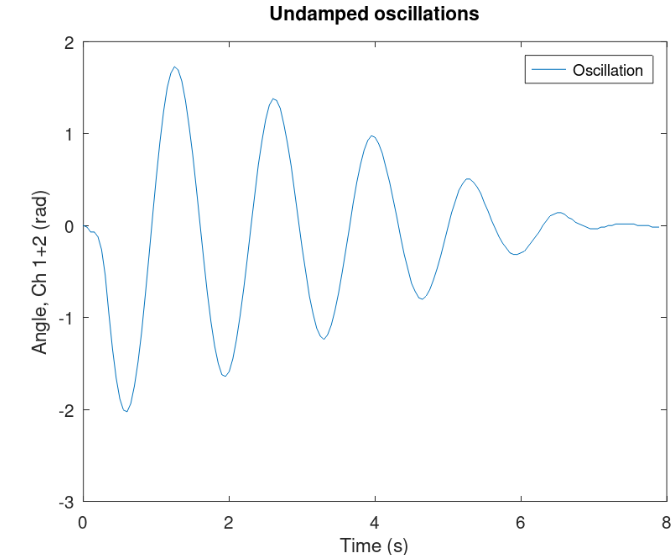
\includegraphics[width=0.6\textwidth]{oscillations/images/Undamped_Oscillations}
  \caption{Oscillations without damping}
  \label{fig:undamped_oscillations}
\end{figure}

From the measurements, the coordinates of the maxima were determined and from this the natural frequency was determined to be $\omega = 4.8 \pm 0.1 (rad/s)$, which was constant throughout the measurements.

\begin{figure}[h!]
  \centering
  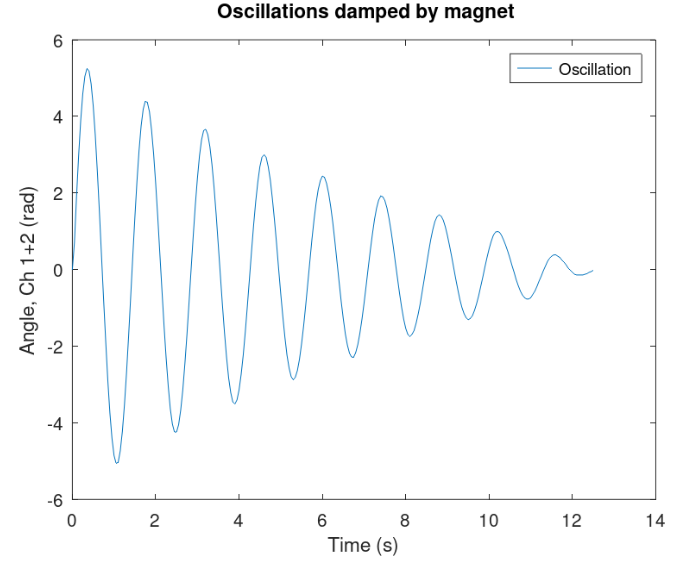
\includegraphics[width=0.6\textwidth]{oscillations/images/underdamped}
  \caption{Decrease in amplitude by an added damping term}
  \label{fig:underdamped}
\end{figure}

A damping term was added by placing the magnet back in its original position, the oscillations are displayed in Figure \ref{fig:underdamped}. The coordinates of nine of the maxima were determined and were plotted in Figure \ref{fig:log of damping factor}. 

\begin{figure}[h!]
  \centering
  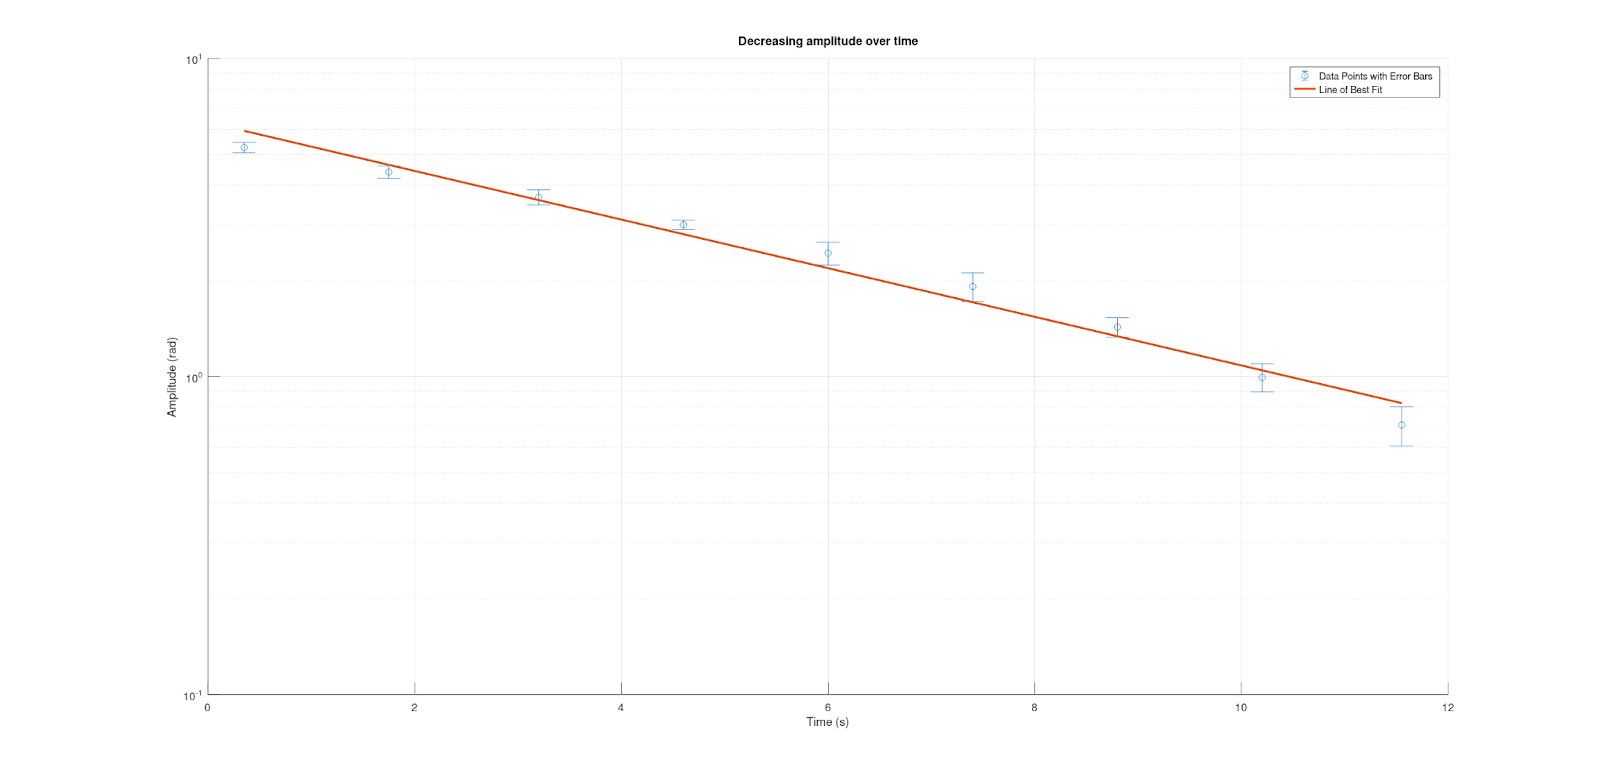
\includegraphics[width=1\textwidth]{oscillations/images/unnamed}
  \caption{Semi-logaritmic plot of the amplitude over time}
  \label{fig:log of damping factor}
\end{figure}

The displacement amplitude $x(t)$ decreases as shown in Eq.~\eqref{eq:underdamped_solution}. The slope of the line of best-fit $m$ is equal to the $-\gamma$ term in Eq.~\eqref{eq:underdamped_solution} ($|m| = \gamma $). By this a damping factor of $\gamma_{direct} = 1.3 \pm 0.2 (rad/s)$ was determined.

\subsection{Indirect calculation of the damping factor.}

\begin{figure}[H]
  \centering
  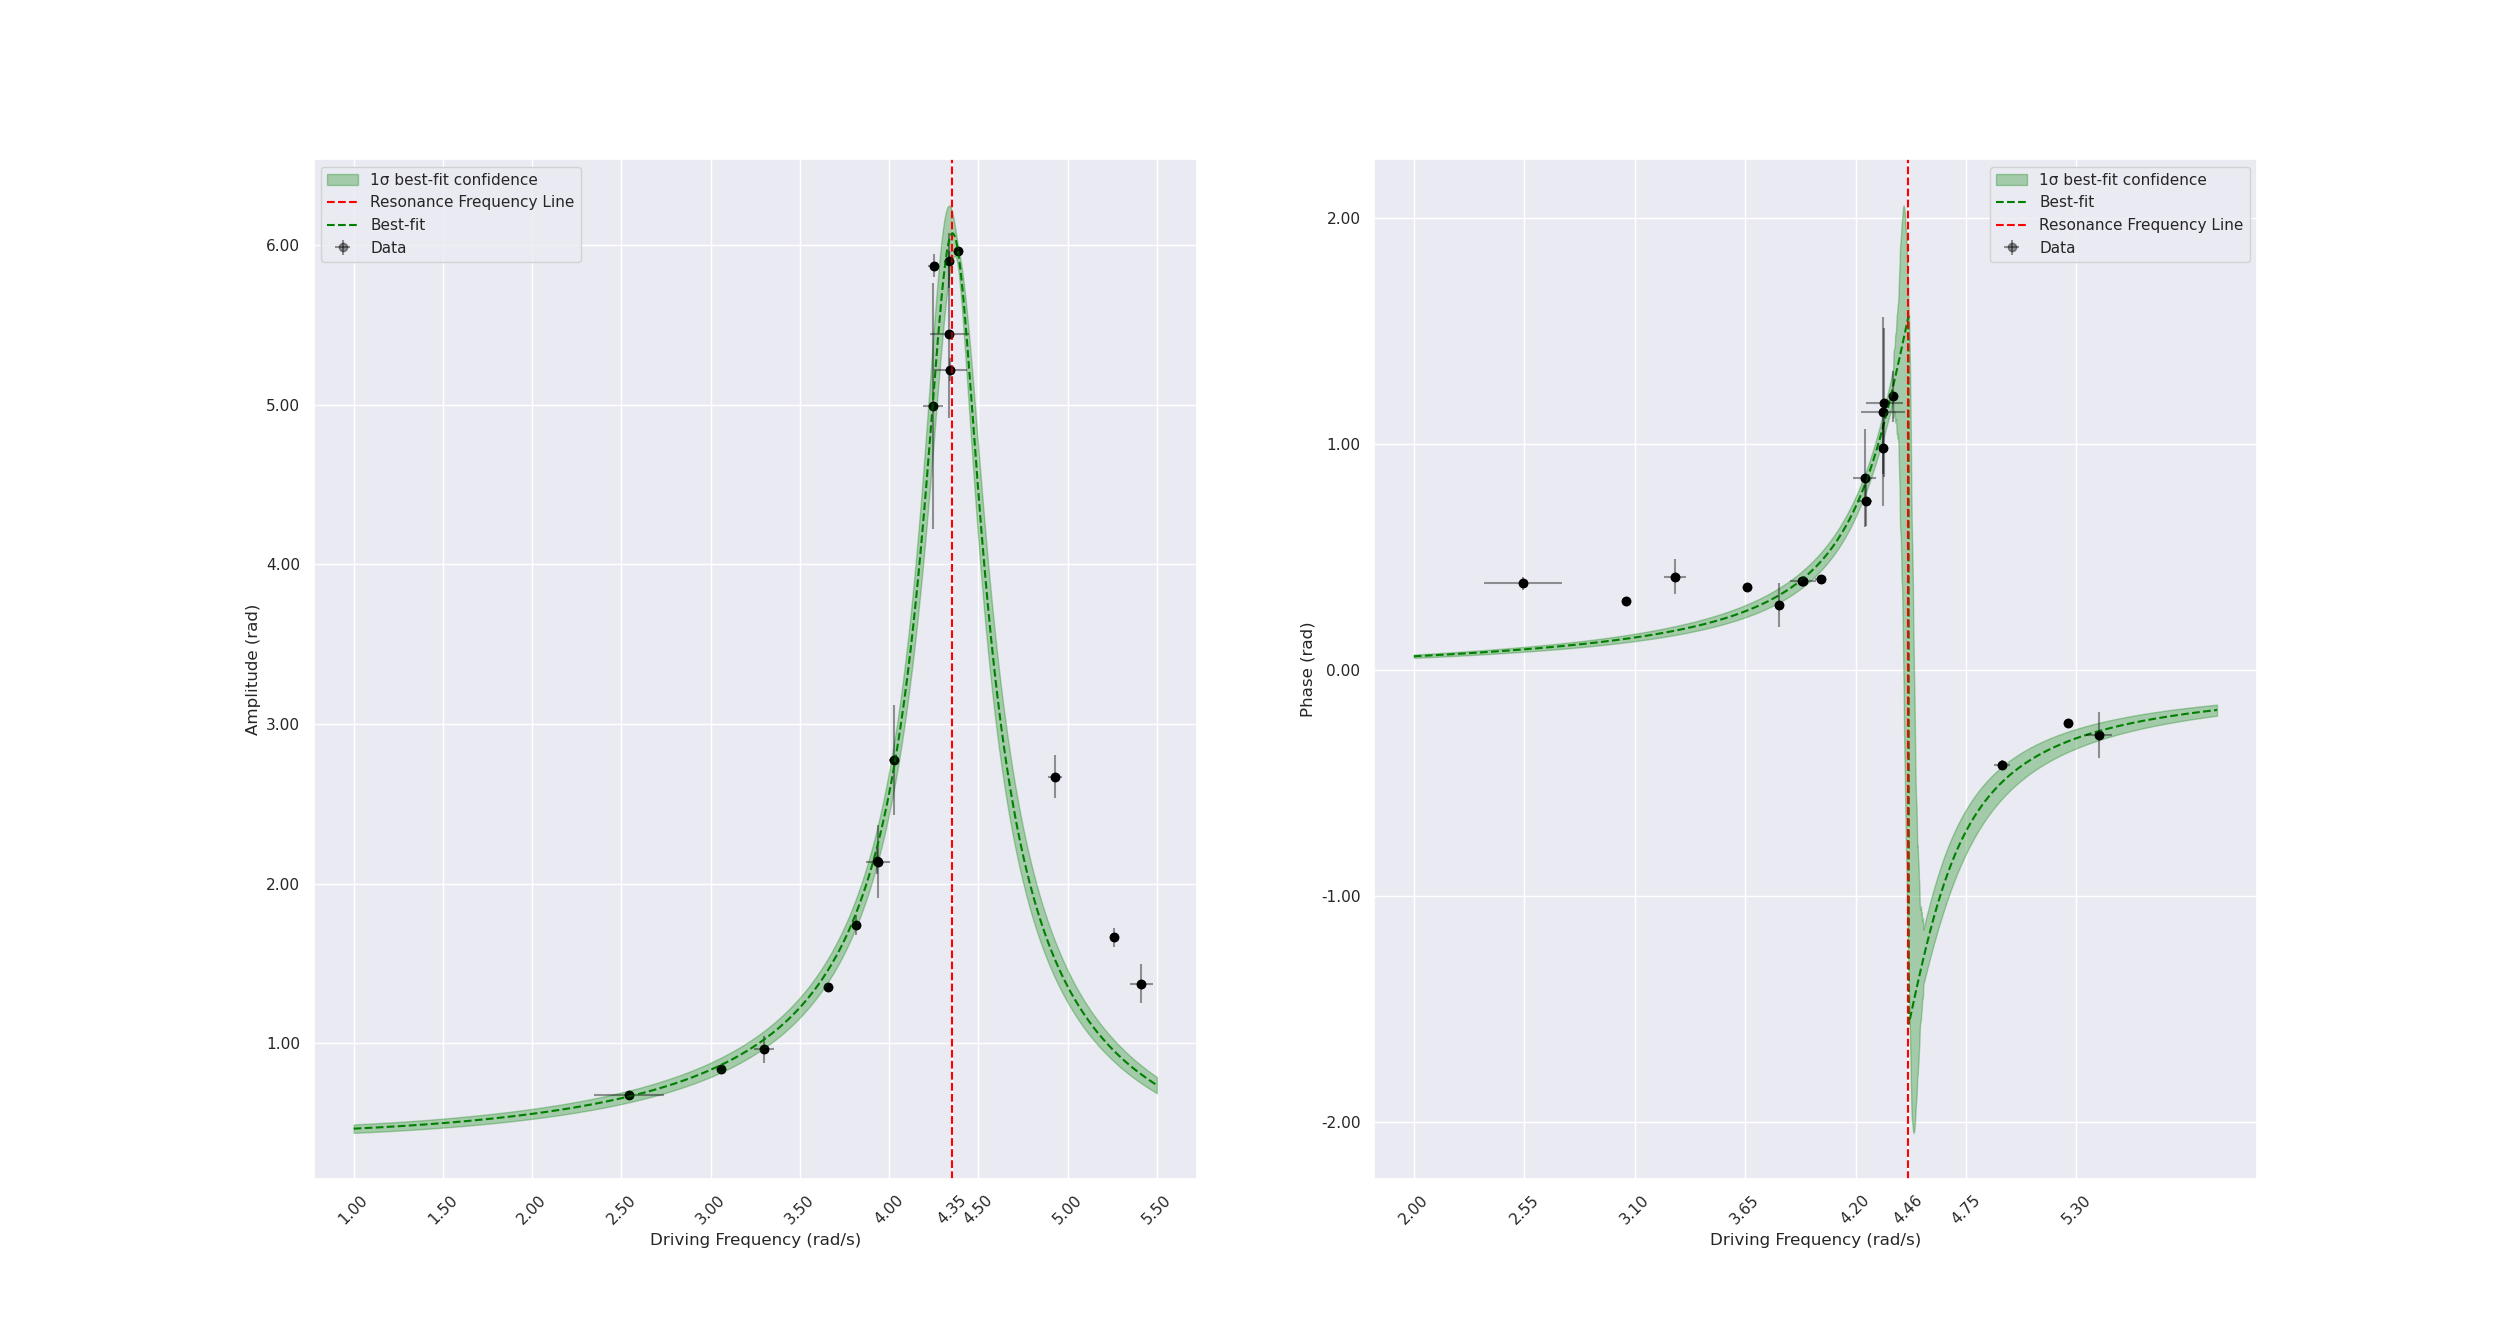
\includegraphics[width=1\textwidth]{oscillations/images/resonance}
  \caption{The amplitude and phase difference of the oscillations plotted against driving frequency.}
  \label{fig:resonance}
\end{figure}

The graph of the amplitude and phase difference of the oscillations against driving frequencies with best-fit curves and correspoding uncertanties are depicted in Figure.\ref{fig:resonance}. Tabular data with respective errors are depicted in Table \ref{tab:data} in appendix \ref{appendix:data}.

Resonance frequency from the amplitude-frequency graph is estimated to be $\omega_{amplitude} = 4.35 \pm 0.09 (rad/s)$. Resonance frequency from the phase-frequency graph is estimated to be $\omega_{phase} = 4.46 \pm 0.02 (rad/s)$. Combined resonance frequency is

\begin{equation*}
\omega_{res} = \frac{\omega_{amplitude} + \omega_{phase}}{2} \pm \sqrt{\Delta\omega_{amplitude}^2 + \Delta\omega_{phase}^2} = 4.4 \pm 0.1 (rad/s)
\end{equation*}

Damping factor is again evaluated from Eq.~\ref{eq:freq_deps}.

\begin{equation*}
        \gamma_{indirect} = \sqrt{ \frac{\omega^2 - \omega_{res}^2}{2} } = \sqrt{ \frac{4.8^2 - 4.4^2}{2} } = 1.3 \pm 0.8 (rad/s)
\end{equation*}       

This damping factor matches the damping factor previously calculated, $\gamma_{direct}$.

Error analysis for the resonance frequencies and the damping factor is located in Appendix \ref{appendix:errors}.
